\subsection{Anwendungen}

\subsubsection{Bannerdemo}

\begin{center}
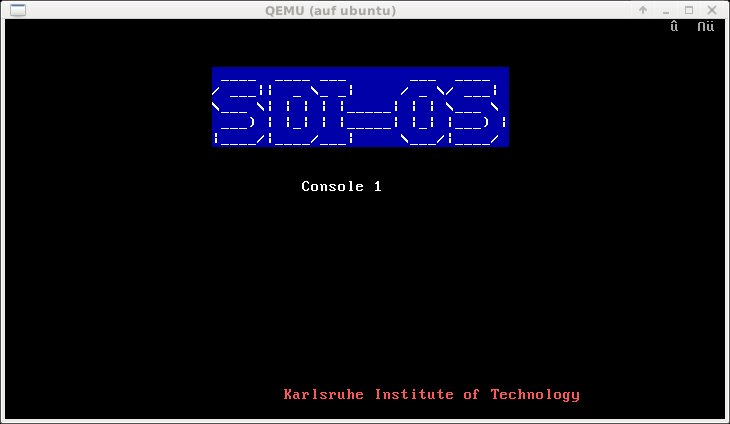
\includegraphics[scale=0.65]{bannerdemo}
\end{center}

Die \textit{Bannerdemo} war die erste Anwendung, welche Ausgaben über den Consoleserver tätigte. Sie zeigt ein einfaches ASCII-Art-Logo, die Nummer der aktuellen Konsole und den Text "Karlsruhe Institute of Technology" als kontinuierlich durchlaufendes Banner.

\subsubsection{Pong}

\begin{center}
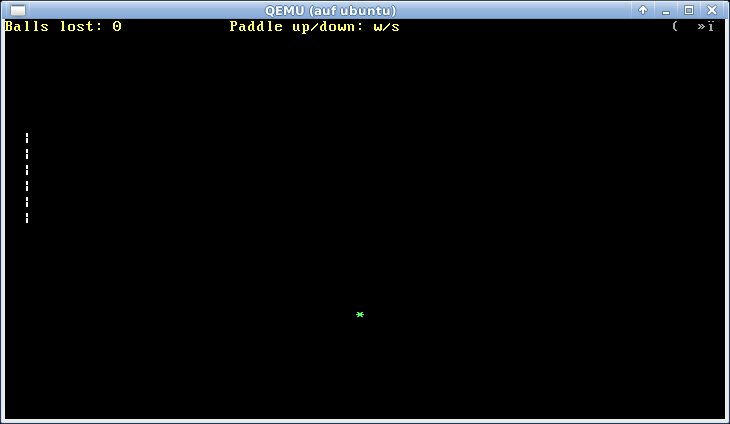
\includegraphics[scale=0.65]{pong}
\end{center}

\textit{Pong} implementiert ein einfaches Pong-Spiel für einen Spieler. Der Ball prallt an der oberen, unteren und rechten Bildschirmgrenze sowie dem Paddel ab und muss mit dem über die Tasten "w" und "s" gesteuerten Paddel darn gehindert werden, an der linken Bildschirmgrenze aus dem Spielfeld zu fallen.